%% ============================================================
%%  STANDARD PREAMBLE (article, lecture notes) -- Quiz 1 of the
%%  phase-diagram course: problems and solutions
%% ============================================================

% ---------- Document class and page layout ----------
\documentclass[11pt]{article}      % Basic document type, 11pt body text
\usepackage[margin=1in]{geometry}  % Sets page margins to 1 inch on all sides

% ---------- Paragraph style ----------
\usepackage{setspace}              % Lets you set the line spacing of the whole document
\setstretch{1.2}                   % Line spacing factor: 1.0 = single (default), 1.2 = slightly airy, 1.5 = very loose
\setlength{\parindent}{2em}        % First-line indent of each paragraph
\setlength{\parskip}{1\baselineskip} % Extra vertical gap between paragraphs
\setlength{\emergencystretch}{3em}  % Extra stretch so long inline math breaks without overfull lines

% ---------- Math ----------
\usepackage{amsmath,amssymb}       % Core math: align, cases, \text{}, \boxed{}, plus extra symbols (\mathbb, \hbar, ...)

% ---------- Figures ----------
\usepackage{graphicx}              % \includegraphics for the pre-built figures in figures/
\usepackage{float}                 % [H] keeps each figure at its place in the text
\usepackage{needspace}             % keeps a problem and its figure on one page

% ---------- Colors and boxes ----------
\usepackage{xcolor}                % Lets you use colors (\textcolor{red}{...})

% ---------- Text layout ----------
\usepackage{indentfirst}           % Indents the first paragraph after a heading (article class skips it by default)

% ---------- Hyperlinks (load last) ----------
\usepackage[hidelinks]{hyperref}   % Clickable TOC, \ref, \eqref, \cite; hidelinks = no colored text or boxes

% ---------- Equation numbering ----------
\numberwithin{equation}{section}   % Equation counter resets in each section
\renewcommand{\theequation}{\thesection.\arabic{equation}} % Displays numbers as section.equation, e.g. (2.3)

% ---------- Figure references in the style of the writing guide ----------
\newcommand{\figref}[1]{Fig.~\ref{#1}}

% ---------- Title block ----------
\title{Phase Diagrams: Quiz 1 with Solutions}
\author{Duy M. Dao}
\date{\today}                      % Compile date; replace with a fixed date if you prefer

\begin{document}
\maketitle                         % Prints title, author, date

% ============================================================
\section{Problems}
% ============================================================

\paragraph{Problem 1.}
The binary system $A$--$B$ forms the congruently melting compound $A_xB_y$.
Alloys between $A$ and $A_xB_y$ are of the eutectic type, and alloys between $A_xB_y$ and $B$ are of the peritectic type.
Draw a phase diagram for this system.
Describe how the percentages of the phases change if the eutectic point moves slightly to the left or to the right.

\needspace{312pt}
\paragraph{Problem 2.}
Figure~\ref{fig:q1-lens} shows an isomorphous system.
A bar of $A$ and a bar of $B$ are joined and heated to $T_2$ for isothermal diffusion.
For the average compositions $x_1$ and $x_2$, state which phases form and give their compositions.

\begin{figure}[H]
\centering
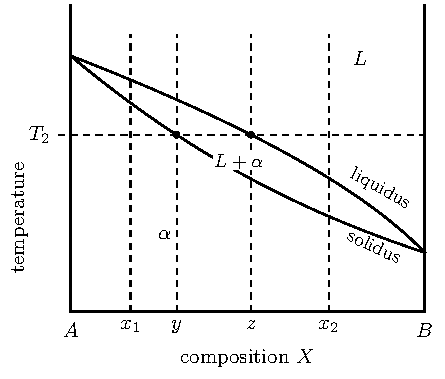
\includegraphics{figures/quiz1_lens}
\caption{Isomorphous system of Problem~2, with the isotherm $T_2$ and the compositions $x_1$, $y$, $z$ and $x_2$.}
\label{fig:q1-lens}
\end{figure}

\needspace{366pt}
\paragraph{Problem 3.}
Figure~\ref{fig:q1-pt} shows the $P$--$T$ projection of a binary system with a quadruple point $Q$ of the eutectoid type.
Draw the $T$--$X$ diagram at the pressure $p_0$.

\begin{figure}[H]
\centering
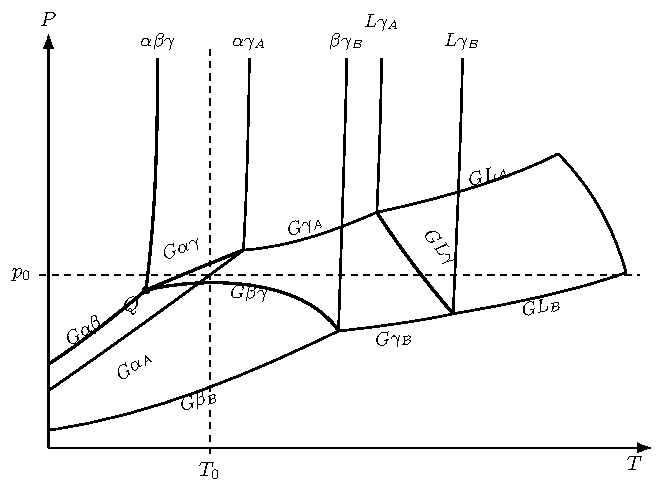
\includegraphics{figures/quiz1_pt}
\caption{$P$--$T$ projection of Problem~3. Thick lines: binary three-phase equilibria. Thin lines: equilibria of the pure components $A$ and $B$. Dashed lines: the isobar $p_0$ and the isotherm $T_0$.}
\label{fig:q1-pt}
\end{figure}

\needspace{344pt}
\paragraph{Problem 4.}
Figure~\ref{fig:q1-agpr} shows the Ag--Pr phase diagram.
List all the three-phase reactions that involve the liquid phase.

\begin{figure}[H]
\centering
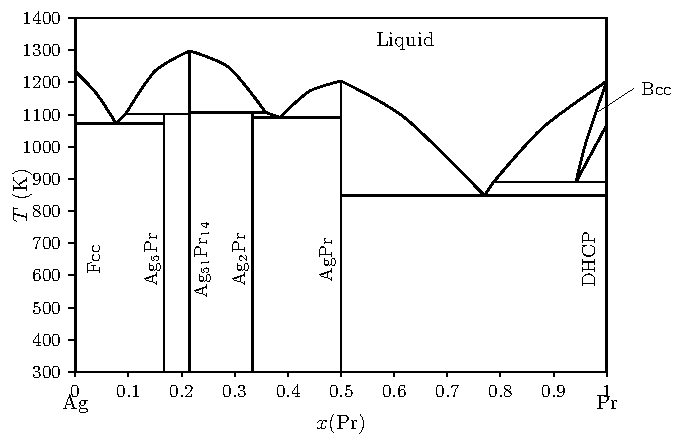
\includegraphics{figures/quiz1_agpr}
\caption{Ag--Pr phase diagram of Problem~4, redrawn from the quiz figure.}
\label{fig:q1-agpr}
\end{figure}

\needspace{369pt}
\paragraph{Problem 5.}
Figure~\ref{fig:q1-tern} shows the diopside--anorthite--albite (Di--An--Ab) system.
The Di--An and Di--Ab sides are binary eutectic systems, and the Ab--An side is a solid-solution loop without a minimum.
Mark the eutectic points, the direction of falling temperature and the three-phase region, and state the meaning of each kind of line.
Draw an isotherm through $l_4$.
For solidification, give the approximate composition of point $A$ and the path of the liquid during the cooling of composition $A$.

\begin{figure}[H]
\centering
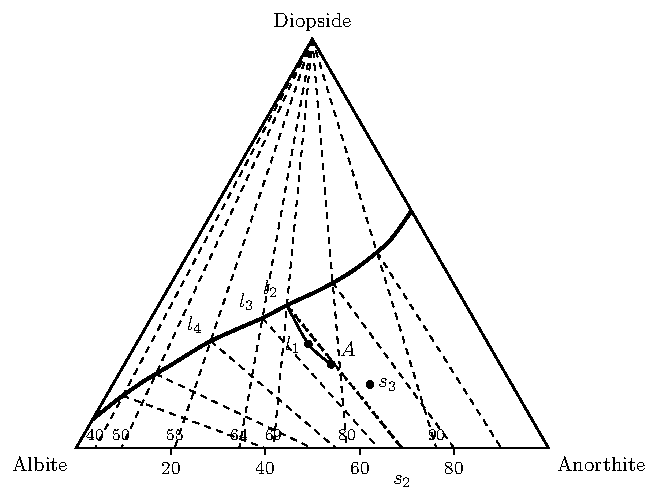
\includegraphics{figures/quiz1_ternary}
\caption{Di--An--Ab system of Problem~5 (compositions in wt\%). Thick curve: cotectic. Dashed lines: diopside--liquid lines and liquid--plagioclase tie lines, with the An content of the plagioclase in equilibrium with each liquid. Solid curve and dotted line: crystallization of composition $A$.}
\label{fig:q1-tern}
\end{figure}

% ============================================================
\section{Solutions}
% ============================================================

\subsection{Problem 1: Compound with a Eutectic and a Peritectic Side}

\paragraph{Construction from two partial diagrams.}
The compound $A_xB_y$, denoted $\gamma$, divides the system into the partial systems $A$--$\gamma$ and $\gamma$--$B$.
Figure~\ref{fig:q1-sol1} shows the diagram assembled from a eutectic diagram for $A$--$\gamma$ and a peritectic diagram for $\gamma$--$B$.
In the $A$--$\gamma$ part, the liquid decomposes at the eutectic temperature $T_E$ into the $A$-rich solid solution $\alpha$ and $\gamma$, $L \to \alpha + \gamma$.
In the $\gamma$--$B$ part, the $B$-rich solid solution $\beta$ has the highest melting point, and the peritectic reaction $L + \beta \to \gamma$ occurs at $T_P$.
The phase $\gamma$ dissolves some $B$, so the $\gamma$ field widens toward $B$ and meets the peritectic isotherm.

\begin{figure}[H]
\centering
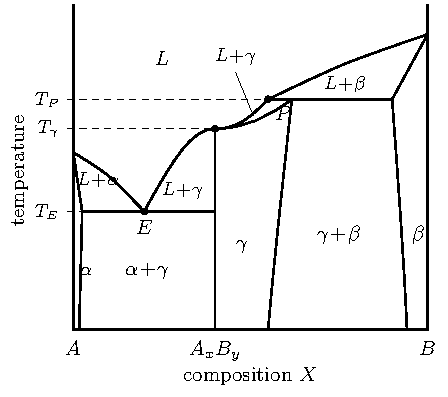
\includegraphics{figures/quiz1_sol_compound}
\caption{Phase diagram for Problem~1. $E$: eutectic point. $P$: liquid composition of the peritectic reaction. Dot at $T_\gamma$: congruent melting point of $A_xB_y$.}
\label{fig:q1-sol1}
\end{figure}

\paragraph{Congruent melting next to a peritectic.}
In a peritectic reaction, the product lies between the two reactants on the isotherm.
For $L + \beta \to \gamma$, the liquid composition $X_P$ therefore lies on the $A$ side of the $\gamma$ composition on the isotherm, between the stoichiometric composition $X_\gamma$ and the $\gamma$ boundary.
A liquid can exist at $X_P$ on the isotherm only if $T_P$ exceeds the melting point $T_\gamma$ of the compound.
The liquidus therefore rises continuously from $E$ through the congruent point $(X_\gamma, T_\gamma)$ to $P$.
The Gibbs--Konovalov relation (Section~11.6 of the notes) requires horizontal tangents where the liquid and the solid have the same composition.
The congruent point of $\gamma$ is therefore a horizontal inflection of the liquidus and not a maximum.
A liquidus maximum at $X_\gamma$ would make the $\gamma$ liquidus fall toward $B$, and no peritectic reaction with only $L$, $\beta$ and $\gamma$ could then form on the $B$ side.
A convex-hull calculation with a compound that dissolves $B$ but not $A$ reproduced this topology.

\paragraph{Total amounts of the phases.}
Consider an alloy of composition $X_0$ between $X_\alpha$ and $X_\gamma$, the compositions of $\alpha$ and $\gamma$ on the eutectic isotherm.
Below $T_E$, the lever rule gives the fractions of the two phases as
\begin{equation}
    n_\alpha = \frac{X_\gamma - X_0}{X_\gamma - X_\alpha},
    \qquad
    n_\gamma = \frac{X_0 - X_\alpha}{X_\gamma - X_\alpha},
\end{equation}
where $n_\alpha$ is the fraction of $\alpha$ and $n_\gamma$ is the fraction of $\gamma$.
These fractions do not contain the eutectic composition $X_E$, so a small shift of the eutectic point leaves the total amounts of $\alpha$ and $\gamma$ unchanged.

\paragraph{Amounts of primary crystals and eutectic.}
The shift changes the microconstituents, which are the primary crystals formed above $T_E$ and the eutectic mixture formed at $T_E$.
For a hypoeutectic alloy, $X_\alpha < X_0 < X_E$, the lever rule on the eutectic isotherm gives
\begin{equation}
    n_{\text{eut}} = \frac{X_0 - X_\alpha}{X_E - X_\alpha},
    \qquad
    n_{\text{prim}} = \frac{X_E - X_0}{X_E - X_\alpha},
\end{equation}
where $n_{\text{eut}}$ is the fraction of eutectic and $n_{\text{prim}}$ is the fraction of primary $\alpha$.
If the eutectic point moves to the right, $X_E$ increases, so the alloy contains more primary $\alpha$ and less eutectic.
The eutectic itself then contains more $\gamma$, with the fraction $(X_E - X_\alpha)/(X_\gamma - X_\alpha)$.
A shift to the left has the opposite effect.
If $X_E$ passes $X_0$, the alloy changes from hypoeutectic to hypereutectic, and primary $\gamma$ replaces primary $\alpha$.
An alloy of the original eutectic composition contains, after a small shift in either direction, a small amount of primary $\alpha$ or primary $\gamma$ in addition to the eutectic.

\subsection{Problem 2: Isothermal Diffusion in an Isomorphous System}

\paragraph{Layers during diffusion.}
At $T_2$, pure $A$ is solid, and pure $B$ is liquid, because $T_2$ lies above the melting point of $B$ (\figref{fig:q1-lens}).
At the joint, $A$ dissolves into the liquid and $B$ diffuses into the solid.
At fixed temperature and pressure, both chemical potentials are constant across a two-phase mixture, so no diffusion flux passes through a two-phase zone.
The $L + \alpha$ region of the diagram therefore appears only as a sharp interface.
The couple consists of a solid $\alpha$ layer with compositions from $0$ to $y$ and a liquid layer with compositions from $z$ to $1$ (\figref{fig:q1-sol2}).
The tie line at $T_2$ fixes the compositions $y$ and $z$ on the two sides of the interface.

\begin{figure}[H]
\centering
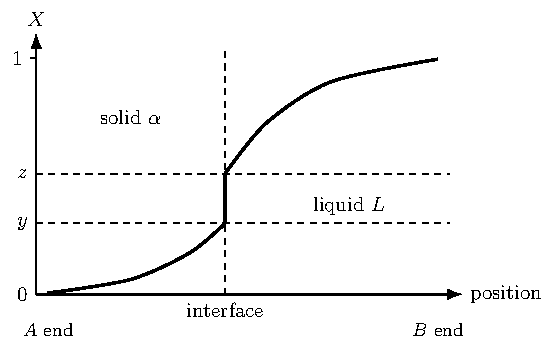
\includegraphics{figures/quiz1_sol_profile}
\caption{Composition profile of the diffusion couple at $T_2$ before the composition becomes uniform.}
\label{fig:q1-sol2}
\end{figure}

\paragraph{Final state.}
Diffusion continues until the composition is uniform.
For the average composition $x_1 < y$, the final state lies in the $\alpha$ field, so the liquid disappears and a single solid $\alpha$ of composition $x_1$ remains.
For the average composition $x_2 > z$, the final state lies in the liquid field, so the solid dissolves completely and a single liquid of composition $x_2$ remains.
Only an average composition between $y$ and $z$ leads to a final mixture of $\alpha$ with composition $y$ and liquid with composition $z$, in the amounts given by the lever rule.

\subsection{Problem 3: $T$--$X$ Diagram from a $P$--$T$ Projection}

\paragraph{Crossings of the isobar.}
In \figref{fig:q1-pt}, the isobar $p_0$ lies above $Q$ and below the triple point of pure $A$ at which $\alpha$, $\gamma$ and gas coexist.
The isobar crosses seven curves, which are listed in Table~\ref{tab:q1-cross} in order of increasing temperature.
Each binary three-phase curve becomes a three-phase isotherm of the $T$--$X$ diagram, and each curve of a pure component becomes a transition point on the side $X = 0$ or $X = 1$.
Pure $A$ forms neither $\gamma$ nor liquid at $p_0$ and sublimes directly at $T_3$.

\begin{table}[htbp]
\centering
\caption{Curves of \figref{fig:q1-pt} crossed by the isobar $p_0$.}
\label{tab:q1-cross}
\renewcommand{\arraystretch}{1.25}
\begin{tabular}{llll}
    \hline
    Temperature & Curve & Equilibrium & Reaction on cooling \\
    \hline
    $T_1$ & $\alpha\beta\gamma$ & binary, three phases & $\gamma \to \alpha + \beta$ (eutectoid) \\
    $T_2$ & $G\alpha\gamma$ & binary, three phases & $G \to \alpha + \gamma$ \\
    $T_3$ & $G\alpha_A$ & pure $A$ & sublimation of $\alpha$ \\
    $T_4$ & $\beta\gamma_B$ & pure $B$ & $\gamma \to \beta$ \\
    $T_5$ & $GL\gamma$ & binary, three phases & $L \to G + \gamma$ \\
    $T_6$ & $L\gamma_B$ & pure $B$ & solidification \\
    $T_7$ & $GL_B$ & pure $B$ & condensation \\
    \hline
\end{tabular}
\end{table}

\paragraph{Type of each three-phase isotherm.}
At $T_1$, the $\gamma$ solid solution decomposes on cooling into $\alpha$ and $\beta$, the eutectoid reaction that defines the type of $Q$.
At $T_2$, gas forms below the sublimation temperature $T_3$ of pure $A$.
The partial pressure of $A$ in a gas that also contains $B$ is smaller than $p_0$, so $\alpha$ coexists with this gas at a lower temperature than with pure $A$ vapor.
The gas is therefore the middle phase, and the reaction on cooling is $G \to \alpha + \gamma$.
At $T_5$, the liquid is the middle phase, and the reaction on cooling is $L \to G + \gamma$, a eutectic-type reaction with a gas phase (Table~5 of the notes).

\paragraph{Assembly of the diagram.}
Figure~\ref{fig:q1-sol3} shows the resulting diagram.
Below $T_1$, the alloys consist of $\alpha$ and $\beta$.
Between $T_1$ and $T_2$, the $\gamma$ field opens in the middle, with $\alpha + \gamma$ and $\gamma + \beta$ on the two sides.
The isotherm at $T_2$ caps the $\alpha + \gamma$ region, and the $\alpha + G$ region rises from this isotherm to the sublimation point of $A$ at $T_3$.
The $\gamma + \beta$ region closes at the transformation point of $B$ at $T_4$.
The $G + \gamma$ region extends from $T_2$ to the isotherm at $T_5$, where the liquid appears.
Above $T_5$, the $L + \gamma$ region closes at the melting point of $B$ at $T_6$, and the $G + L$ region closes at the boiling point of $B$ at $T_7$.
Two two-phase regions lie above each three-phase isotherm and one lies below, as required for eutectic-type reactions.

\begin{figure}[H]
\centering
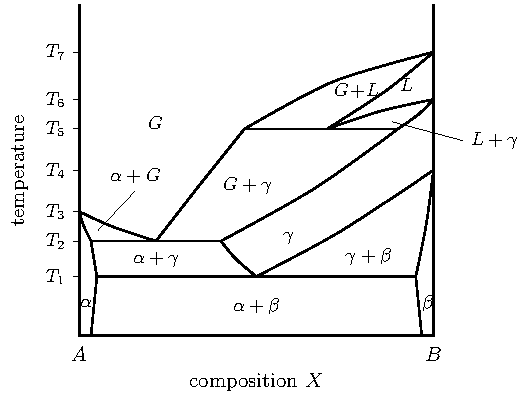
\includegraphics{figures/quiz1_sol_tx}
\caption{Schematic $T$--$X$ diagram at the pressure $p_0$. $T_1$ to $T_7$: crossings of the isobar listed in Table~\ref{tab:q1-cross}.}
\label{fig:q1-sol3}
\end{figure}

\subsection{Problem 4: Three-Phase Reactions in the Ag--Pr System}

\paragraph{Identification of the reactions.}
Each horizontal line of \figref{fig:q1-agpr} that touches the liquidus is a three-phase isotherm with liquid.
The type of each reaction follows from the middle phase on the isotherm.
A liquid in the middle gives a eutectic, a solid compound in the middle gives a peritectic, and a solid in the middle that decomposes into liquid and another solid on cooling gives a metatectic.
The compositions and temperatures in Table~\ref{tab:q1-agpr} were read from the diagram, with an accuracy of $\pm 10$~K and $\pm 0.01$ in $x$(Pr).

\begin{table}[htbp]
\centering
\caption{Three-phase reactions with liquid in the Ag--Pr system.}
\label{tab:q1-agpr}
\renewcommand{\arraystretch}{1.25}
\begin{tabular}{llcc}
    \hline
    Reaction on cooling & Type & $T$ (K) & $x_L$(Pr) \\
    \hline
    $L \to \text{Fcc(Ag)} + \text{Ag}_5\text{Pr}$ & eutectic & 1072 & 0.08 \\
    $L + \text{Ag}_{51}\text{Pr}_{14} \to \text{Ag}_5\text{Pr}$ & peritectic & 1102 & 0.10 \\
    $L + \text{Ag}_{51}\text{Pr}_{14} \to \text{Ag}_2\text{Pr}$ & peritectic & 1107 & 0.36 \\
    $L \to \text{Ag}_2\text{Pr} + \text{AgPr}$ & eutectic & 1091 & 0.39 \\
    $\text{Bcc(Pr)} \to L + \text{DHCP(Pr)}$ & metatectic & 890 & 0.79 \\
    $L \to \text{AgPr} + \text{DHCP(Pr)}$ & eutectic & 848 & 0.77 \\
    \hline
\end{tabular}
\end{table}

\paragraph{Two-phase equilibria with liquid.}
The compounds Ag$_{51}$Pr$_{14}$ and AgPr melt congruently, at 1298~K and 1204~K, and pure Ag melts at 1235~K and pure Pr at 1204~K.
These equilibria involve only two phases and are therefore not three-phase reactions.
The transformation of pure Pr from Bcc to DHCP at 1068~K involves no liquid.

\subsection{Problem 5: The Diopside--Anorthite--Albite System}

\paragraph{Eutectic points and falling temperature.}
The two binary eutectics lie on the sides of the triangle (\figref{fig:q1-sol5}).
The eutectic $E_1$ on the Di--An side lies at 58~wt\% Di and 42~wt\% An, and the eutectic $E_2$ on the Di--Ab side lies close to the Ab corner, at 7~wt\% Di.
The Ab--An side has no minimum, so the system has no ternary eutectic.
Temperature falls along the cotectic from $E_1$ to $E_2$, along the Ab--An side from An to Ab, and in each primary field from the Di corner or the An corner toward the cotectic.

\begin{figure}[H]
\centering
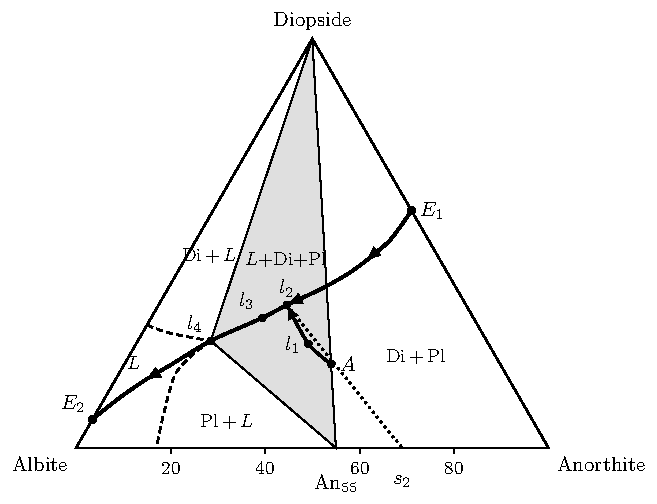
\includegraphics{figures/quiz1_sol_ternary}
\caption{Solution of Problem~5. Arrows on the cotectic: direction of falling temperature. Shaded triangle: three-phase field at the temperature of $l_4$. Dashed curve through $l_4$: isotherm. Thick arrow: path of the liquid for composition $A$.}
\label{fig:q1-sol5}
\end{figure}

\paragraph{Meaning of the lines.}
The thick curve is the cotectic, along which the liquid is saturated with both diopside and plagioclase.
The dashed lines from the Di corner are diopside--liquid tie lines, and their extensions to the Ab--An side mark the projection of each liquid from the Di corner.
The dashed lines from the cotectic to the Ab--An side are liquid--plagioclase tie lines, and each number gives the An content of the plagioclase in equilibrium with the liquid.
The solid curve from $A$ through $l_1$ to $l_2$ is the path of the liquid while plagioclase crystallizes alone.
The dotted line through $l_2$, $A$ and $s_2$ is the tie line at the moment the liquid reaches the cotectic, and the point $s_3$ is the bulk composition of the diopside and plagioclase crystallized when the liquid is at $l_3$.

\paragraph{Three-phase region and the isotherm through $l_4$.}
For each liquid on the cotectic, diopside, the liquid and plagioclase form a tie triangle, and these triangles together make up the three-phase region $L + \text{Di} + \text{Pl}$.
At the temperature of $l_4$, the tie triangle connects Di, $l_4$ and plagioclase An$_{55}$, shaded in \figref{fig:q1-sol5}.
The isotherm through $l_4$ has two branches, one in the diopside field to the Di--Ab side and one in the plagioclase field to the Ab--An side.
The two branches form a V whose vertex at $l_4$ points toward higher temperature along the cotectic.
At this temperature, the liquid field lies toward the Ab corner, the fields Di $+$ $L$ and Pl $+$ $L$ lie on the two sides of the triangle, and the field Di $+$ Pl lies between the triangle and the An corner.

\paragraph{Composition $A$ and the path of the liquid.}
Point $A$ lies at 20~wt\% Di, 44~wt\% An and 36~wt\% Ab, read from \figref{fig:q1-tern} with an accuracy of 2~wt\%.
Point $A$ lies in the plagioclase field, so plagioclase crystallizes first.
The plagioclase is richer in An than the liquid, and the liquid moves away from the plagioclase along the curved path from $A$ through $l_1$ to $l_2$.
The path curves because the plagioclase becomes richer in Ab as the temperature falls.
At $l_2$, the liquid reaches the cotectic in equilibrium with plagioclase $s_2$ (An$_{69}$).
Diopside then crystallizes together with plagioclase, and the liquid moves down the cotectic from $l_2$ through $l_3$ to $l_4$ while the plagioclase becomes more albitic.
Equilibrium crystallization ends at $l_4$, where the join between Di and the plagioclase passes through $A$.
The final plagioclase is An$_{55}$, the ratio $\text{An}/(\text{An} + \text{Ab})$ of composition $A$, and the solid contains 20~wt\% diopside and 80~wt\% plagioclase.
For fractional crystallization, the liquid continues down the cotectic beyond $l_4$ toward $E_2$.

\end{document}
